% !TEX root = ../thesis.tex

\chapter{Virtual Private Network -- VPN}\label{1}
Virtuálna privátna sieť (ďalej \textbf{\acrshort{vpn}}) je jeden zo spôsobov prepojenia zariadení, tak že internetová komunikácia medzi nimi je privátna, resp. zabezpečená aj v prípade používania nezabezpečenej, verejnej siete. Bezpečnosť spojenia je docielená pomocou kryptografických protokolov v tuneli, ktorý VPN vytvára. 
Táto technológia patrí aktuálne k najpoužívanejším spôsobom pripojenia sa medzi 2 rôznymi internetovými doménami. Najčastejší výskyt je možné sledovať v korporačnom prostredí, pričom cieľom je rozšírenie možností bezpečného pripojenia sa k firemnej sieti. Vzhľadom na firemné tajomstvá je nutné aby bolo takéto spojenie bezpečné a zamestnanci sa mohli pripojiť z rôznych miest. Vďaka uvedeným vlastnostiam je následne možná aj práca z~domu (z~ang. \textit{Home office}), ktorá môže byť benefitom pre obe strany. Ukážka použitia VPN je znázornená pomocou \ref{vpndemo}. 
\begin{figure}[!ht]
	\centering
	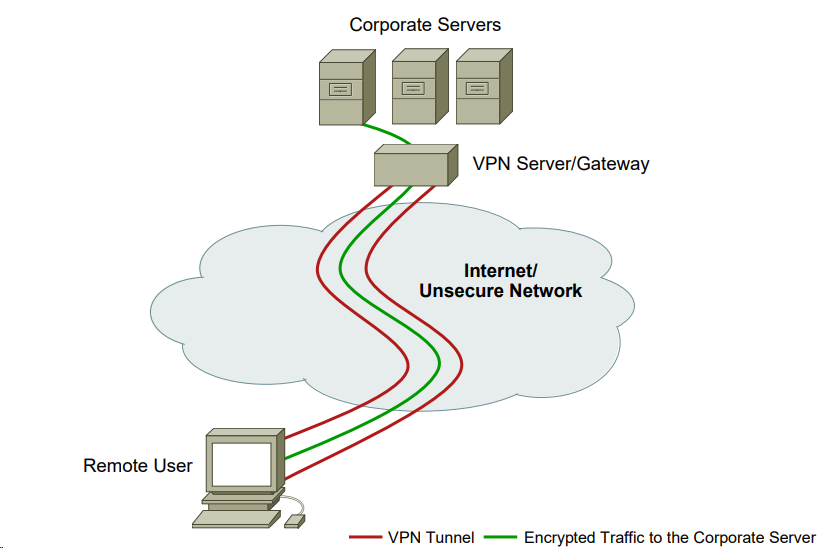
\includegraphics[width=.9\textwidth]{figures/VPNdemo}
	\caption{Ukážka typického VPN pripojenia}
	\label{vpndemo}
\end{figure}

\section{Rozdelenie VPN}
\cite{divvpn}, \cite{ciscovpn}

\section{Protokol riadenia prenosu -- \acrshort{tcp}}
Protokol riadenia prenosu (z ang. \textit{Transmission Control Protocol}, ďalej \acrshort{tcp}) je komunikačný protokol orientovaný na nadviazanie a udržanie sieťového spojenia medzi zariadeniami. Môže byť použitý pri úlohe príjímateľa aj odosielateľa (z ang. \textit{full-duplex}). Úlohou je spoľahlivý prenos dát medzi komunikantmi. Odoslanie a príjem dát je v rovnakom poradí. Protokol zároveň obsahuje mechanizmy na kontrolu výskytu chýb. 

Na začiatku 21. storočia je 95\% paketov používaných na internete TCP. Bežné aplikácie používajúce TCP sú webové (HTTP/HTTPS protokoly), slúžiace na e-mailovú komunikáciu (SMTP/POP3/IMAP) a prenos súborov (z ang. \textit{File Transfer Protocol -- \acrshort{ftp}}). Minimálna dĺžka hlavičky TCP je 20 bajtov a maximálna dĺžka 60 bajtov. Po pridaní údajov TCP hlavičky k prenášaným dátam, vzniká tzv. \textit{segment}. TCP je použitý s internetovým protokolom (ďalej \acrshort{ip}) Z uvedeného dôvodu sa preto často stretávame s označením TCP/IP. Dôležité je však poznamenať, že sa jedná o jeden a ten istý TCP protokol. 

V súvislosti s TCP/IP sa používateľ môže stretnúť s modelom. Ten je zobrazený pomocou schémy \ref{tcpipprot}. V uvedenej schéme sú znázornené aj niektoré z protokolov, ktoré ja na jednotlivých vrstvách používajú.

\begin{figure}[!ht]
	\centering
	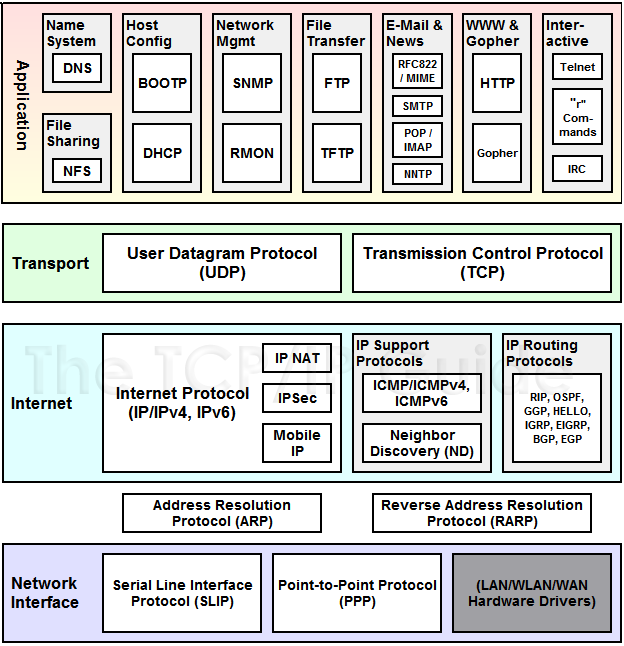
\includegraphics[width=0.9\textwidth]{figures/tcpipprot}
	\caption{Schéma TCP/IP modelu s niektorými protokolmi}
	\label{tcpipprot}
\end{figure}

V súčasnosti je možne TCP protokol implementovať softvérovo aj hardvérovo. Pri prvom z uvedených je problémom závislosť na OS a následne aj vysoká vyťaženosť procesora pri príprave a spracovaní dát. Pri hardvérovom riešení je výhodou optimalizácia a implementácia bez potreby dodatočnej úpravy OS. Hardvérové implementácie sa realizujú pomocou koprocesorov umiestnených vo vnútri procesora. Následkom toho môžeme dnes bežne pozorovať umiestnenie spomenutých zariadení na našich zariadeniach.

Podrobnejšie informácie o TCP protokole je možné nájsť na \cite{tcp2}. V uvedenej publikácií sa nachádza opis TCP hlavičky, metódy nadviazania a ukončenia spojenia. Obdobne je spomenuté ako dochádza k prenosu dát pomocou sekvenčných čísel. Ak má používateľ nejasnosti v fungovaní TCP protokolu, odporúča sa danú publikáciu prečítať.

\section{Kryptografické zabezpečenie protokolov}
TCP protokol sam o sebe nezabezpečí dáta, ku ktorým sa pridáva TCP hlavička. Dôsledkom toho vznikli viacere protokoly slúžiace na autentizované šifrovanie dát. Najznámejší je protokol zabezpečenia prenosu -- \acrshort{tls} a IPSec.
\subsection{Transport Layer Security -- TLS}
Zabezpečenie dát bolo prvotne vykonávané pomocou protokolu \textit{Secure Sockets Layer} -- \acrshort{ssl}. Tento spôsob používa certifikáty na odšifrovanie dát. SSL malo od svojho vytvorenia dlhý vývoj, ktorý smeroval až k doteraz najpoužívanejšiemu TLS vo verzii 1.3. Inými slovami, TLS protokol je nástupca SSL pričom obsahuje rôzne úpravy a vylepšenia najmä z hľadiska rýchlosti. Zároveň sa v dnešnej dobe neodporúča používanie SSL protokolu. Dôsledkom optimalizácií je, že klienta komunikujúci so serverom cez HTTPS protokol s TLS 1.3 je rýchlejší ako v prípade použitia nešifrovaného HTTP variantu. 

TLS pracuje niekde na pomedzi aplikačnej a transportnej vrstvy. Spôsob spracovania dát je zobrazený pomocou schémy \ref{ssl} s SSL operáciami, prebratej z \cite{biks}. 
\begin{figure}[!ht]
	\centering
	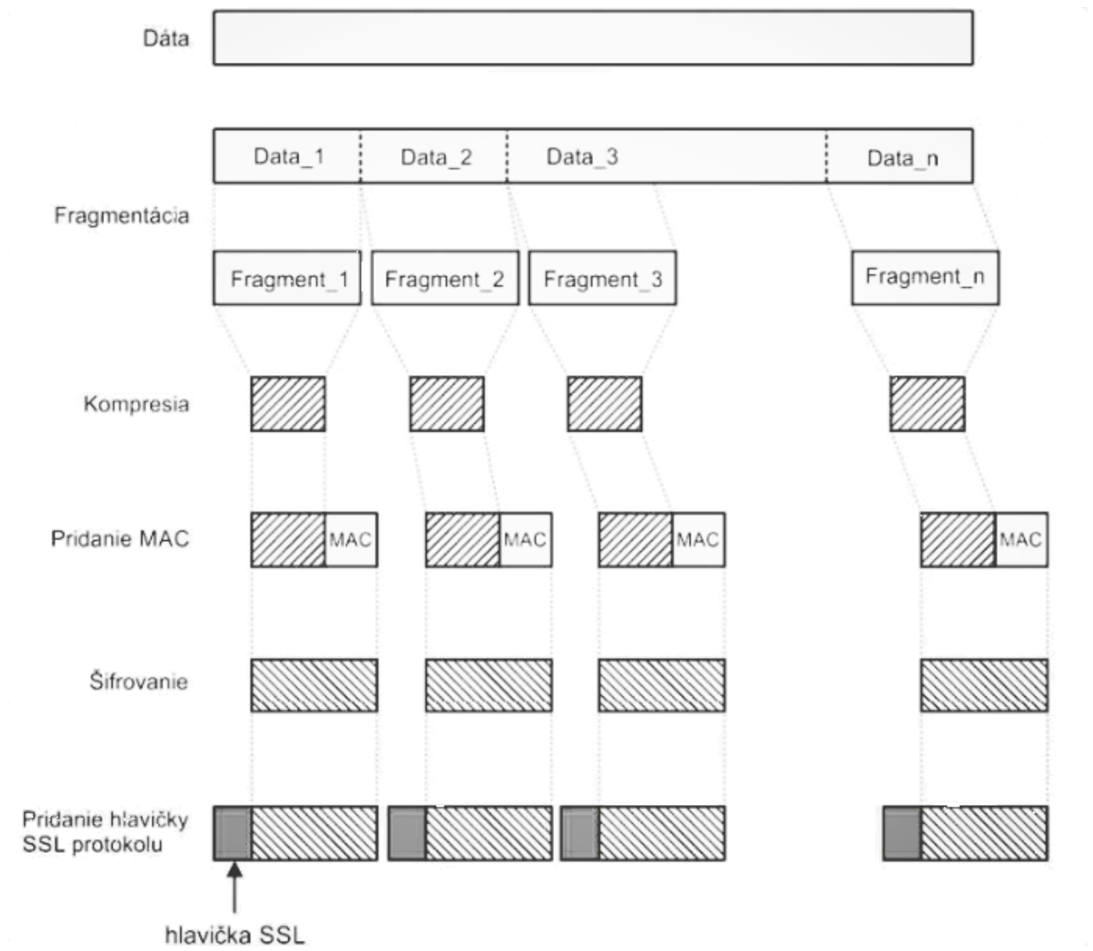
\includegraphics[width=0.7\linewidth]{figures/ssl}
	\caption{Prehľad operácií v SSL protokole}
	\label{ssl}
\end{figure}

Viac informácií o TLS protokole, jednotlivých verziách a optimalizáciách je možné nájsť na \cite{tls}. 

\subsection{Internet Protocol Security  -- IPSec}
Ochrana medzi transportnou a sietovou vrstvou TCL/IP.
Nabudúce. \cite{biks}
\chapter{Kryptografia vo VPN}\label{krypto}
Cieľom kryptografických blokov je utajiť správu pri jej ceste z bodu A do B. Teda od odosielateľa (tvorcu) správy, až k jej príjimateľovi. Dôsledkom tohto úkonu dochádza k zabezpečeniu 3 hlavných úloh kryptografie:
\begin{itemize}
	\item \textbf{Ochrana osobných údajov} (dôvernosť) -- z ang. \textit{Data Privacy}, 
	\item \textbf{Autenticita údajov} (prišla z miesta, kde sa uvádza)  -- z ang. \textit{Data Authenticity},
	\item \textbf{Integrita údajov} (nebola upravovaná na ceste)  -- z ang. \textit{Data Integrity}.
\end{itemize}

 Prvý z uvedených bodov je najčastejšie žiadaným a známym cieľom. Odosielateľ správy zašifruje jej obsah pomocou použitia niektorého z šifrovacích algoritmov, kryptografického kľúča a následne správu odošle. Na druhej strane, príjmateľ, musí použiť komplementárny dešifrovací algoritmus s prislúchajúcim kľúčom. Ktokoľvek kto sa dostane medzi týchto komunikantov, k takto preposielanej správe, z nej nedokáže obsahovo nič zistiť, v istom časovom období. 
 
 Dôsledkom týchto faktov je jasné, že komunikanti musia mať jasne definovaný použitý algoritmus. Zároveň je nutné aby došlo k výmene kryptografických kľúčov, ktoré sú pri šifrovaní a dešifrovaní aplikované. Tým sa zabezpečí aj druhá úloha -- Autenticita dát, pretože potrebné informácie budú mať len komunikanti. 
 
 V kryptografických blokoch sú taktiež aplikované algoritmy na overenie integrity správ. Ich úlohou je potvrdiť, že do obsahu správy nebolo, počas jej transportu medzi komunikantmi, nič pridané, resp. ubrané.
 
 V súčasnosti má používateľ možnosť vybrať si zo širokej ponuky kryptografických algoritmov. Medzi najznámejší patrí \acrshort{aes}  \cite{aes}, ktorý je aktuálne používaný ako štandardný kryptografický algoritmus pri počítačovej komunikácií. Detailný opis jednotlivých blokov a postupov použitých v AES-e, je obsahom rôznych knižných vydaní. Pre čitateľa preto posúvam knihu \cite{levicky}, ktorá obsahuje okrem opisu AES-u aj doležité informácie, týkajúce sa kryptografických základov.

V rámci tejto práce sme sa rozhodli opísať, v súčásnosti menej známe, algoritmy: 
\begin{itemize}
	\item XOODOO \cite{tkecak}
	\item Gimli \cite{gimli}
	\item Simpira384 \cite{simpira}
\end{itemize}  
Uvedené permutácie sú použité ako kryptografické primitívum a pri následnej tvorbe ďalších kryptografickych blokov. 

\section{Kryptografický algoritmus XOODOO a variácie} 
XOODOO je sada 384-bitových kryptografických permutácií parametrizovaných počtom kôl. Funkcia kola/rundy\footnote{z ang. \textit{round}} funguje na 12 slovách\footnote{z ang. \textit{words}} po 32 bitoch, vďaka čomu je efektívna aj na procesoroch nižšej triedy. Vytvoril ju tím Keccak, ktorý stojí za viacerými úspešnými kryptografickými algoritmami. Napríklad hashovacie funkcie z rodiny SHA-3 a iné -- \cite{kecsup}. XOODOO algoritmus vznikol po vytvorení tzv. Kravatte autentizačno-šifrovacieho algoritmu \cite{kravatte}, založené na Keccak-p permutácií \cite{keccakp}. Ten sa ukázal ako dostatočne rýchly na širokom spektre platforiem. Avšak nezapadá do kategórie tzv. ľahkej kryptografie \footnote{z ang. \textit{lightweight cryptography}}.

Tím Keccak vypracoval nové riešenie. Ním bol port medzi ich prvotným Keccak-p dizajnom a Gimli-ho \cite{bernstein2017gimli} permutačným algoritmom. Vo výsledku autori zlúčili lepšie realizované prvky z oboch algoritmov do jedného celku. Primárny problém samotnej Gimli permutácie bol v slabom prejave zmeny výstupu po malých zmenách vo vstupnej správe. Táto vlastnosť sa v kryptografii označuje pomocou anglického pojmu, tzv. \textit{propagation proporties}\footnote{Cieľom je aby aj zmena jedného bitu na vstupe, ovplyvnila čo najviac bitov vo výstupe -- tzv. \textit{Lavínový efekt}.}. Novo-vzniknuté riešenie autori pomenovali XOODOO. Na základe rôznych variácií tohto kryptografického primitíva sa im následne podarilo vytvoriť sadu vysoko efektívnych kryptografických funkcií. 
Medzi sady, ktorých jadro tvorí XOODOO, patrí Xoodyak a Xoofff. Xoofff pozostáva zo zlúčenia Farfalle konštrukcie \cite{farfalle} so XOODOO permutáciou. 

Xoodyak ma narozdiel od Xoofff duplexovú konštrukciu \cite{duplex}. Vo výsledku máme ľahko prenosnú, všestrannú, kryptografickú knižnicu. Je vhodná do výkonovo obmedzených prostredí. Môže sa použiť pre väčšinu kryptografických funkcií, ktoré používajú symetrický kľúč. Napríklad hashovanie, šifrovanie, výpočet MAC alebo autentizované šifrovanie. O kvalite riešenia napovedá aj fakt, že sada Xoodyak je jedným z 10 finalistov v oblasti ľahkej kryptografie NIST štandardizačného procesu.
V rámci tejto kapitoly opíšeme kryptografické primitívum XOODOO a následne balík Xoodyak. Informácie o téme boli čerpané z týchto zdrojov: \cite{tkecak}, \cite{xd}, \cite{xcb}, \cite{xoodoocb}, \cite{xdupdate},\cite{xdr1}.
\subsection{XOODOO permutácia}
XOODOO je rodina permutácií, ktorá je definovaná počtom rúnd. Má klasickú iteračnú štruktúru. Teda opakovateľne sa vola rundová funkcia s aktuálnym stavom. Pre pochopenie operácií je nutné pochopiť určité označenie použité v algoritme.

Stav -- \textbf{state}, pozostáva z 3 rovnako veľkých horizontálnych rovín -- \textbf{planes}. Každá z týchto rovín obsahuje štyri paralelne 32-bitové pruhy -- \textbf{lanes}. Okrem tejto charakteristiky je možné opísať stav ako množinu 128 stĺpcov -- \textbf{columns}, pričom jeden stĺpec obsahuje 3 bity v každej rovine. Stav je teda tvorený zo stĺpcov usporiadaných v poli o rozmere 4x32. Posledná položka na opis stavu sú tzv. listy -- \textbf{sheets}. List sa skladá z 3 na sebe uložených pruhov. Uvedené pojmy sú znázornené pomocou schémy \ref{xoodooterm}, ktorá bola prebraná z \cite{xcb}.

\begin{figure}[!h]
	\centering
	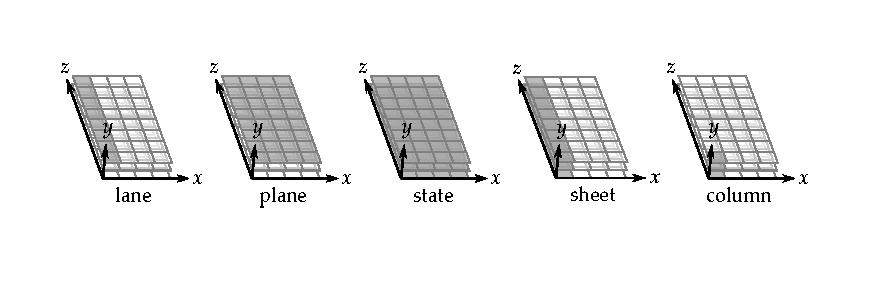
\includegraphics[width=1\textwidth]{figures/xoodooTerminology}
	\caption{Grafické znázornenie terminológie v XOODOO}
	\label{xoodooterm}
\end{figure}

Roviny majú index $y$. $y=0$ zodpovedá spodnej rovine a vrchná rovina $y=2$. Bit je označený s indexom $z$ vrámci množiny pruhov. List ich označujeme pomocou indexu $x$. Takže pozícia pruhu v stave je definovaná pomocou dvoch súradníc $(x,y)$. Konkrétny bit je možné v stave následne reprezentovať pomocou trojice súradníc $(x,y,z)$. Pri učení stĺpca sú potrebné 2 súradnice $(x,z)$. Pred spustením samotného algoritmu musí používateľ vykonať mapovanie 384-bitovej správy voči horizontálnym rovinám. Tento úkon sa realizuje pomocou matematickej formuly \ref{index}.

\begin{equation}\label{index}
	i=z+32(x+4y)
\end{equation}

Rundová funkcia pozostáva z 5 krokov:
\begin{enumerate}
	\item a	mixing layer $\theta$, 
	\item a plane shifting $\rho_{west}$, 
	\item the addition of round constants $\iota$,
	\item a non-linear layer $\chi$,
	\item an another plane shifting $\rho_{east}$.
\end{enumerate}
Celý algoritmus je znázornený pomocou schémy \ref{xoodooalgo}, ktorá je prebratá z \cite{xcb}. 

  \begin{figure}[!h]
  	\centering
  	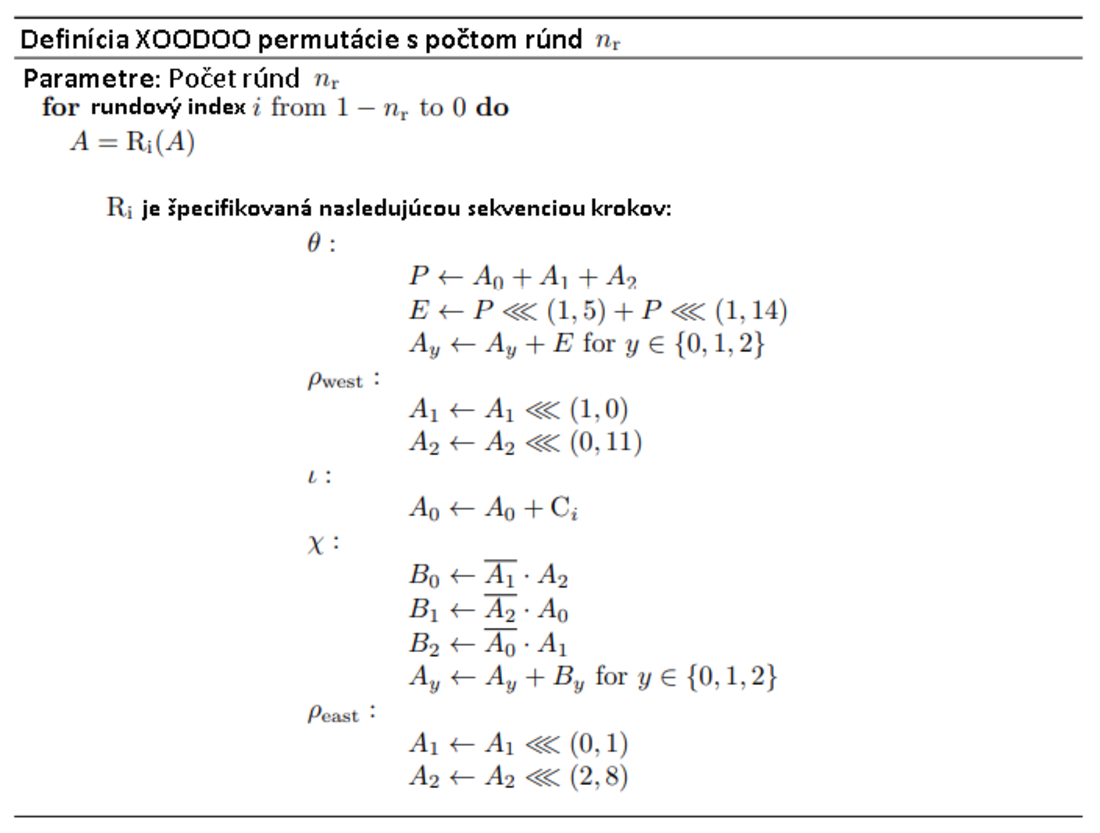
\includegraphics[width=1.1\textwidth]{figures/xoodooalgo}
  	\caption{}
  	\label{xoodooalgo}
  \end{figure}

\subsection{Xoodyak} 
Xoodyak možno považovať za všestranný kryptografický nástroj. Je vhodný pre väčšinu operácií využívajúcich symetrický kľúč. Napríklad generovanie pseudonáhodných bitov, autentizáciu, šifrovanie a mnohé iné. Tím Keccak použil pri návrhu duplexnú konštrukciu. Konkrétne variant s plným stavom a využitím kľúča. Tento dizajn označujeme ako \acrfull{fskd}. Viac o tejto konštrukcii si čitateľ môže prečítať v \cite{duplex}.
Operačný režim, v ktorom Xoodyak pracuje sa nazýva Cyklista -- z ang. \textit{Cyclist}. Tento názov získal ako opozitum k pomenovaniu režimu Motorista, ktorý je možné nájsť v Keyak schéme \cite{keyak}. Narozdiel od uvedeného balíka Keyak, nie je Xoodyak limitovaný len na autentizované šifrovanie. Je jednoduchší hlavne kvôli tomu že neobsahuje paralelné varianty.

\subsubsection{Režim Cyklista}\label{cyklista}
Režim Cyklista funguje na princípe kryptografických permutácií $f$, teda zmeny usporiadania bitov za pomoci tajného kľúča a matematických operácií. Parametrami sú veľkosti blokov $R_{hash}$, $R_{kin}$, $R_{kout}$ a veľkosť račety, resp. západky\footnote{z ang. \textit{the ratchet size}} \cite{ratchet} $\ell_{ratchet}$. Uvedený pojem sa v kryptografii používa vo forme obrazného pomenovania. Cieľom je poukázať na jednoduchý pohyb vpred, ale s ťažkým, resp. zložitejším pohybom naspäť. Dôležité je, že uvedený scenár je vyvolaný zámerným dizajnom. Šírka permutácie $b'$ je definovaná pomocou matematickej formuly \ref{index2}. Všetky uvedené parametre sú v bajtoch. Pre označenie prázdneho slova budeme používať $\epsilon$.
\begin{equation}\label{index2}
	max(R_{hash}, R_{kin}, R_{kout}) + 2 \leq b'
\end{equation} 

Cyklista operuje v dvoch režimoch -- \textbf{hašovací a kľúčový}\footnote{z ang. \textit{hash and keyed mode}.}. 
Inicializácia prebieha pomocou príkazu \lstinline|CYCLIST(K,id,counter)|. Ak sa parameter $K$ rovná prázdnemu slovu $\epsilon$, tak potom nastane spustenie v hašovacom režime. Aktuálne nie je do implementácie zakomponovaná možnosť zmeny režimu po inicializácií. Vývojári však túto vlastnosť nevylúčili pre prípadné aktualizácie balíka.  


Dostupné funkcie závisia od režimu, v ktorom sa  Cyklista spúšťa. Medzi ne patria \lstinline|ABSORB()| a \lstinline|SQUEEZE()|. Možno ich volať v oboch režimoch, zatiaľ čo funkcie \lstinline|ENCRYPT()|, \lstinline|DECRYPT()|, \lstinline|SQUEEZEKEY()| a \lstinline|RATCHET()| sú dostupné len pre kľúčový režim. Účel každej funkcie je nasledujúci:
\begin{itemize}
	\item \lstinline|ABSORB(X)| absorbuje vstupný reťazec X,
	\item C $\gets$ \lstinline|ENCRYPT(P)| zašifruje P do C a absorbuje P,
	\item P $\gets$ \lstinline|DECRYPT(C)| dešifruje C do P a absorbuje P,
	\item Y $\gets$	\lstinline|SQUEEZE($\ell$)|  vytvára $\ell$-bajtový výstup, ktorý závisí od doteraz absorbovaných dát,
	\item Y $\gets$	\lstinline|SQUEEZEKEY($\ell$)| funguje ako \lstinline|SQUEEZE($\ell$)|, ale používa sa za účelom generovania odvodeného kľúča, 		\\ell nefunguje v listings pckg
	\item \lstinline|RATCHET()| transformuje stav na nevratný tak, aby sa zabezpečila dopredná bezpečnosť\footnote{z ang. \textit{Forward secrecy}} \cite{fsec}. 
\end{itemize}

Stav bude závisieť od postupnosti volaní funkcií a od jeho vstupných reťazcov. Presnejšie povedané, zámerom je, že akýkoľvek výstup závisí od postupnosti všetkých vstupných reťazcov a volaní, tak že akékoľvek dva nasledujúce výstupné reťazce budú výstupom rôznych domén. Napríklad volanie \lstinline|ABSORB(X)| znamená, že výstup bude závisieť od reťazca $X$. Na druhej strane \lstinline|ABSORB()| vo funkcii \lstinline|ENCRYPT(P)| vytvorí výstup závislý aj od $P$ z funkcie šifrovania. Okrem uvedených závislostí ovplyvňujú výstup aj iné dizajnové riešenia. Príkladom je minimalizácia pamäťovej stopy. Vo výsledku teda výstup závisí od počtu predchádzajúcich volaní funkcie \lstinline|SQUEEZE()| a predtým spracovaných textov pomocou funkcií \lstinline|ENCRYPT()| a \lstinline|DECRYPT()|. Viac informácií o režime je dostupných v kapitole 7.2, publikácie \cite{xcb}. 

\subsubsection{Definícia a bezpečnosť}
Xoodyak je definovaný pomocou operatívneho režimu Cyklista nasledovne:
\begin{equation}
	CYCLIST[f,R_{hash},R_{kin},R_{kout},\ell_{ratchet}]
\end{equation} 
Kde jednotlivé parametre majú veľkosti:
\begin{enumerate}
	\item $f$ -- permutácia XOODOO so šírkou 48 bajtov (384 bitov),
	\item $R_{hash}$ -- 16 bajtov,
	\item $R_{kin}$ -- 44 bajtov,
	\item $R_{kout}$ -- 24 bajtov,
	\item $\ell_{ratchet}$ -- 16 bajtov.  
\end{enumerate}
Takto definované parametre algoritmu dokážu poskytnúť 128-bitovú bezpečnosť v oboch režimoch Cyklistu. Samozrejmosťou je, že v prípade kľúčového režimu, musí byť veľkosť kľúča rovná alebo väčšia ako 128 bitov. Viac informácií o kryptografickej bezpečnosti algoritmov je možné nájsť v \cite{sec}.

Viac informácií o bezpečnosti Xoodyak-a je možné nájsť v \cite{xcb, 7.3}, odkiaľ boli informácie čerpané.

\subsection{Možnosti použitia Xoodyak algoritmu}
Obsahom tejto podkapitoly sú uvedené postupy ako a za akých okolností je daný balík možné použiť. 
\subsubsection{Použitie hašovacieho režimu}
Xoodyak sa dá aplikovať ako hašovacia funkcia.
\subsubsection{Použitie kľúčového režimu}
\section{Kryptografický algoritmus Gimli} 
\section{Kryptografický algoritmus Simpira384} 
